% !TEX root = ../thesis.tex
% simulation processes and execution
% @author Tobias Wulf
%

\section{Simulationsprozesse und Ausführung}\label{sec:sim-pro}


In diesem Abschnitt der Arbeit werden Ausführungen zum Gesamtsimulationsbetriebs und zur Moduleinbindung anhand von Prozessdarstellungen und Blockschemata erläutert. Jeder Simulationsabschnitt wird getrennt betrachtet. Prozesse und Schemata beziehen sich auf die Implementierung in den Anhängen und die dort beschriebenen Algorithmen. Gleichzeitig wird entsprechender Bezug zur Software-Dokumentation hergestellt, sodass ausgeführte Implementierungen zu umgesetztem Quellcode referenzierbar wird.


\subsection{Sensor-Array-Simulation}\label{sub:sensor-array-pro}


Das Sensor-Array-Simulationsmodul \autoref{mcode:sensorarraysimulation} ist funktional aufgebaut. Geschriebener Quellcode des Moduls mündet in eine Hauptsimulationsfunktion, siehe \autoref{mcode:simulatedipolesquaresensorarray}. Diese ist mittels Skripten nach \autoref{fig:blockschemasensor-array} für den Simulationsbetrieb inklusive Konfiguration und Kennfelddatensatz zu laden.

\vspace{2mm}
\begin{figure}[bph]
	\centering
	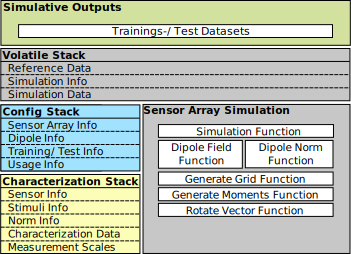
\includegraphics[width=0.7\linewidth]{chapters/images/3-SW-E-OExp/Blockschema_Sensor-Array}
	\caption[Blockschema Einbindung der Sensor-Array-Simulation]{Blockschema Einbindung der Sensor-Array-Simulation. Das Schema beschreibt die Quellcodeeinbindung des Sensor-Array-Simulationsmodul für eine Ausführung mittels Skript-Dateien. Das Modul ist über die Modulsimulationsfunktion im Skript ausgeführt. Der Simulationsfunktion werden geladene Datensätze als entsprechende Simulations-Stacks zugeführt. Innerhalb die Funktions-Workspace sind alle Simulationsergebnisse prozessiert und zyklisch in Trainings-/ Testdatensätze zu speichern.}
	\label{fig:blockschemasensor-array}
\end{figure}


\clearpage


Das ausführende Skript der Simulation ist im \autoref{mcode:generatesimulationdatasets} zu finden. Es werden jeweils Trainings- und Testdatensätze gemäß eingestellter Konfiguration prozessiert. Die Sichtung der Datensätze und eine Analyse der Rohdaten ist mit Plot-Funktionen des \autoref{mcode:plotfunctions} durchzuführen. Die Plot-Funktionen können direkt ausgeführt werden. Eine Auswahl der zu sichtenden Daten ist über Nutzereingaben in der Konsole gesteuert. Erstellte Datensätze und Plots können mit Lösch-Skripten aus \autoref{mcode:deletesimulationdatasets} und \autoref{mcode:deletesimulationplots} entfernt werden.
\newline
Die Simulationsausführung nach \autoref{alg:sensor-array-sim} mittels Skript aus \autoref{mcode:generatesimulationdatasets} ist nochmals zur Verdeutlichung des Ablaufs als Prozess in \autoref{fig:sensor-array-simulation} dargestellt. Als erstes sind alle notwendigen Datensätze in den Skript-Workspace zu laden und als Eingabeargumente der Simulationsfunktion zuzuführen. 


\vspace{5mm}
\begin{figure}[bph]
	\centering
	\includegraphics[width=\linewidth]{chapters/images/3-SW-E-OExp/Sensor-Array-Simulation}
	\caption[Sensor-Array-Simulation Prozessansicht]{Sensor-Array-Simulation Prozessansicht. Prozessabfolge entsprechend der Implementierung aus \autoref{ch:sensor-array-sim-imp} und Ausführung mit Skripten aus \autoref{mcode:executable-scripts} in Kombination mit Datensätzen (DS) nach \autoref{ch:tdk-datensatz} bzw. \autoref{mcode:datasets}.}
	\label{fig:sensor-array-simulation}
\end{figure}


\clearpage


Innerhalb der Funktion folgt eine schrittweise Initialisierung der Simulation nach eingestellter Konfiguration. Es werden Daten-Container angelegt, die Metadaten (Info) der Simulation und prozessierte Simulationsdaten (Data) beinhalten. Die Simulation erfolgt für fest eingestellte Sensor, Magnet-, Rotationsparameter in Training-/ Testdaten und Verkippung. Die räumliche Lage des Sensor-Arrays ist dynamisch über Positionsvektoren in der Konfiguration gesteuert. So wird eine Positionsdrift des Arrays bei gleichbleibende Simulationsparameter umgesetzt. Die Simulation ist in verschachtelten For-Schleifen eingebettet. Die äußeren Schleifen setzen die Positionsdrift um. Die innere Schleife fährt die Magnetrotation durch. Für jede Position wird ein Datensatzpaar aus Trainings-/ Testdaten gespeichert, dass die volle Rotation enthält. Entsprechend des Schleifendurchlaufs werden Info- und Data-Container aktualisiert. Anzahl der Rotationswinkel können für Trainings und Testdaten unterschiedlich eingestellt werden. Ebenfalls können unterschiedliche Rotationsauflösungen und Startphasen parametriert werden, siehe \autoref{mcode:generateconfigmat}.


\subsection{Gauß-Prozess-Regression}\label{sub:gpr-pro}


Für die Verarbeitung von simulierten Sensor-Array-Datensätzen aus \autoref{sub:sensor-array-pro}, dient das Quellcodemodule der Gauß-Prozess-Regression in \autoref{mcode:gaussianprocessregression}. Es ist funktional aufgebaut und erzeugt Regressionsmodelle in einer Trainingsphase. Ein erzeugtes Modell bildet zusammen mit einen Sensor-Array-Datensatz die Eingabeargumente für eine Arbeitsphase. In dieser werden Winkelvorhersagen auf Basis des Sensor-Array-Datensatzes berechnet. Das Quellcodemodul setzt sich aus drei weiteren Submodulen zusammen:


\begin{enumerate}
	\item Mathematische Grundfunktionen, \autoref{mcode:basicmathfunctions}
	\item Kovarianzfunktion f. $d_F^2$ \autoref{eq:kfun} (Matrixdaten), \autoref{mcode:kernelqfc}
	\item Kovarianzfunktion f. $d_E^2$ \autoref{eq:kfun} (Vektordaten), \autoref{mcode:kernelqfcapx}
\end{enumerate}


Erläuterungen zur Einbindung von Trainingsphase und Arbeitsphase folgen zusammenfassend wie in \autoref{sub:sensor-array-pro} und beziehen sich auf das Demonstrationsskript für die Gauß-Prozess-Regression im \autoref{mcode:demogprmodule}. Das Demonstrationsskript bedingt ein Trainings- und Testdatensatzpaar, dass mit gleichen Simulationsparametern in Bezug auf Position und Verkippung erstellt worden ist.


\clearpage


\paragraph{Trainingsphase}\label{par:gpr-training-pro}$~$\\


Die Bildung des Regressionsmodell in der Trainingsphase ist modular nach \autoref{fig:blockschematrainingsphase} umgesetzt. Einstiegspunkt für die optimierte Modellerstellung nach \autoref{alg:bayesopt} ist die Funktion in \autoref{mcode:optimgpr}. Diese entspricht der Implementierung in \autoref{sec:gpropt}. Der Funktion werden zuvor geladene Konfigurationen sowie Trainings- und Testdaten zugeführt. Als Rückgabe erfolgt das optimierte Regressionsmodell mit der Fähigkeit zur Winkelvorhersage auf Basis von weiteren Testdatensätzen.


\vspace{3mm}
\begin{figure}[bph]
	\centering
	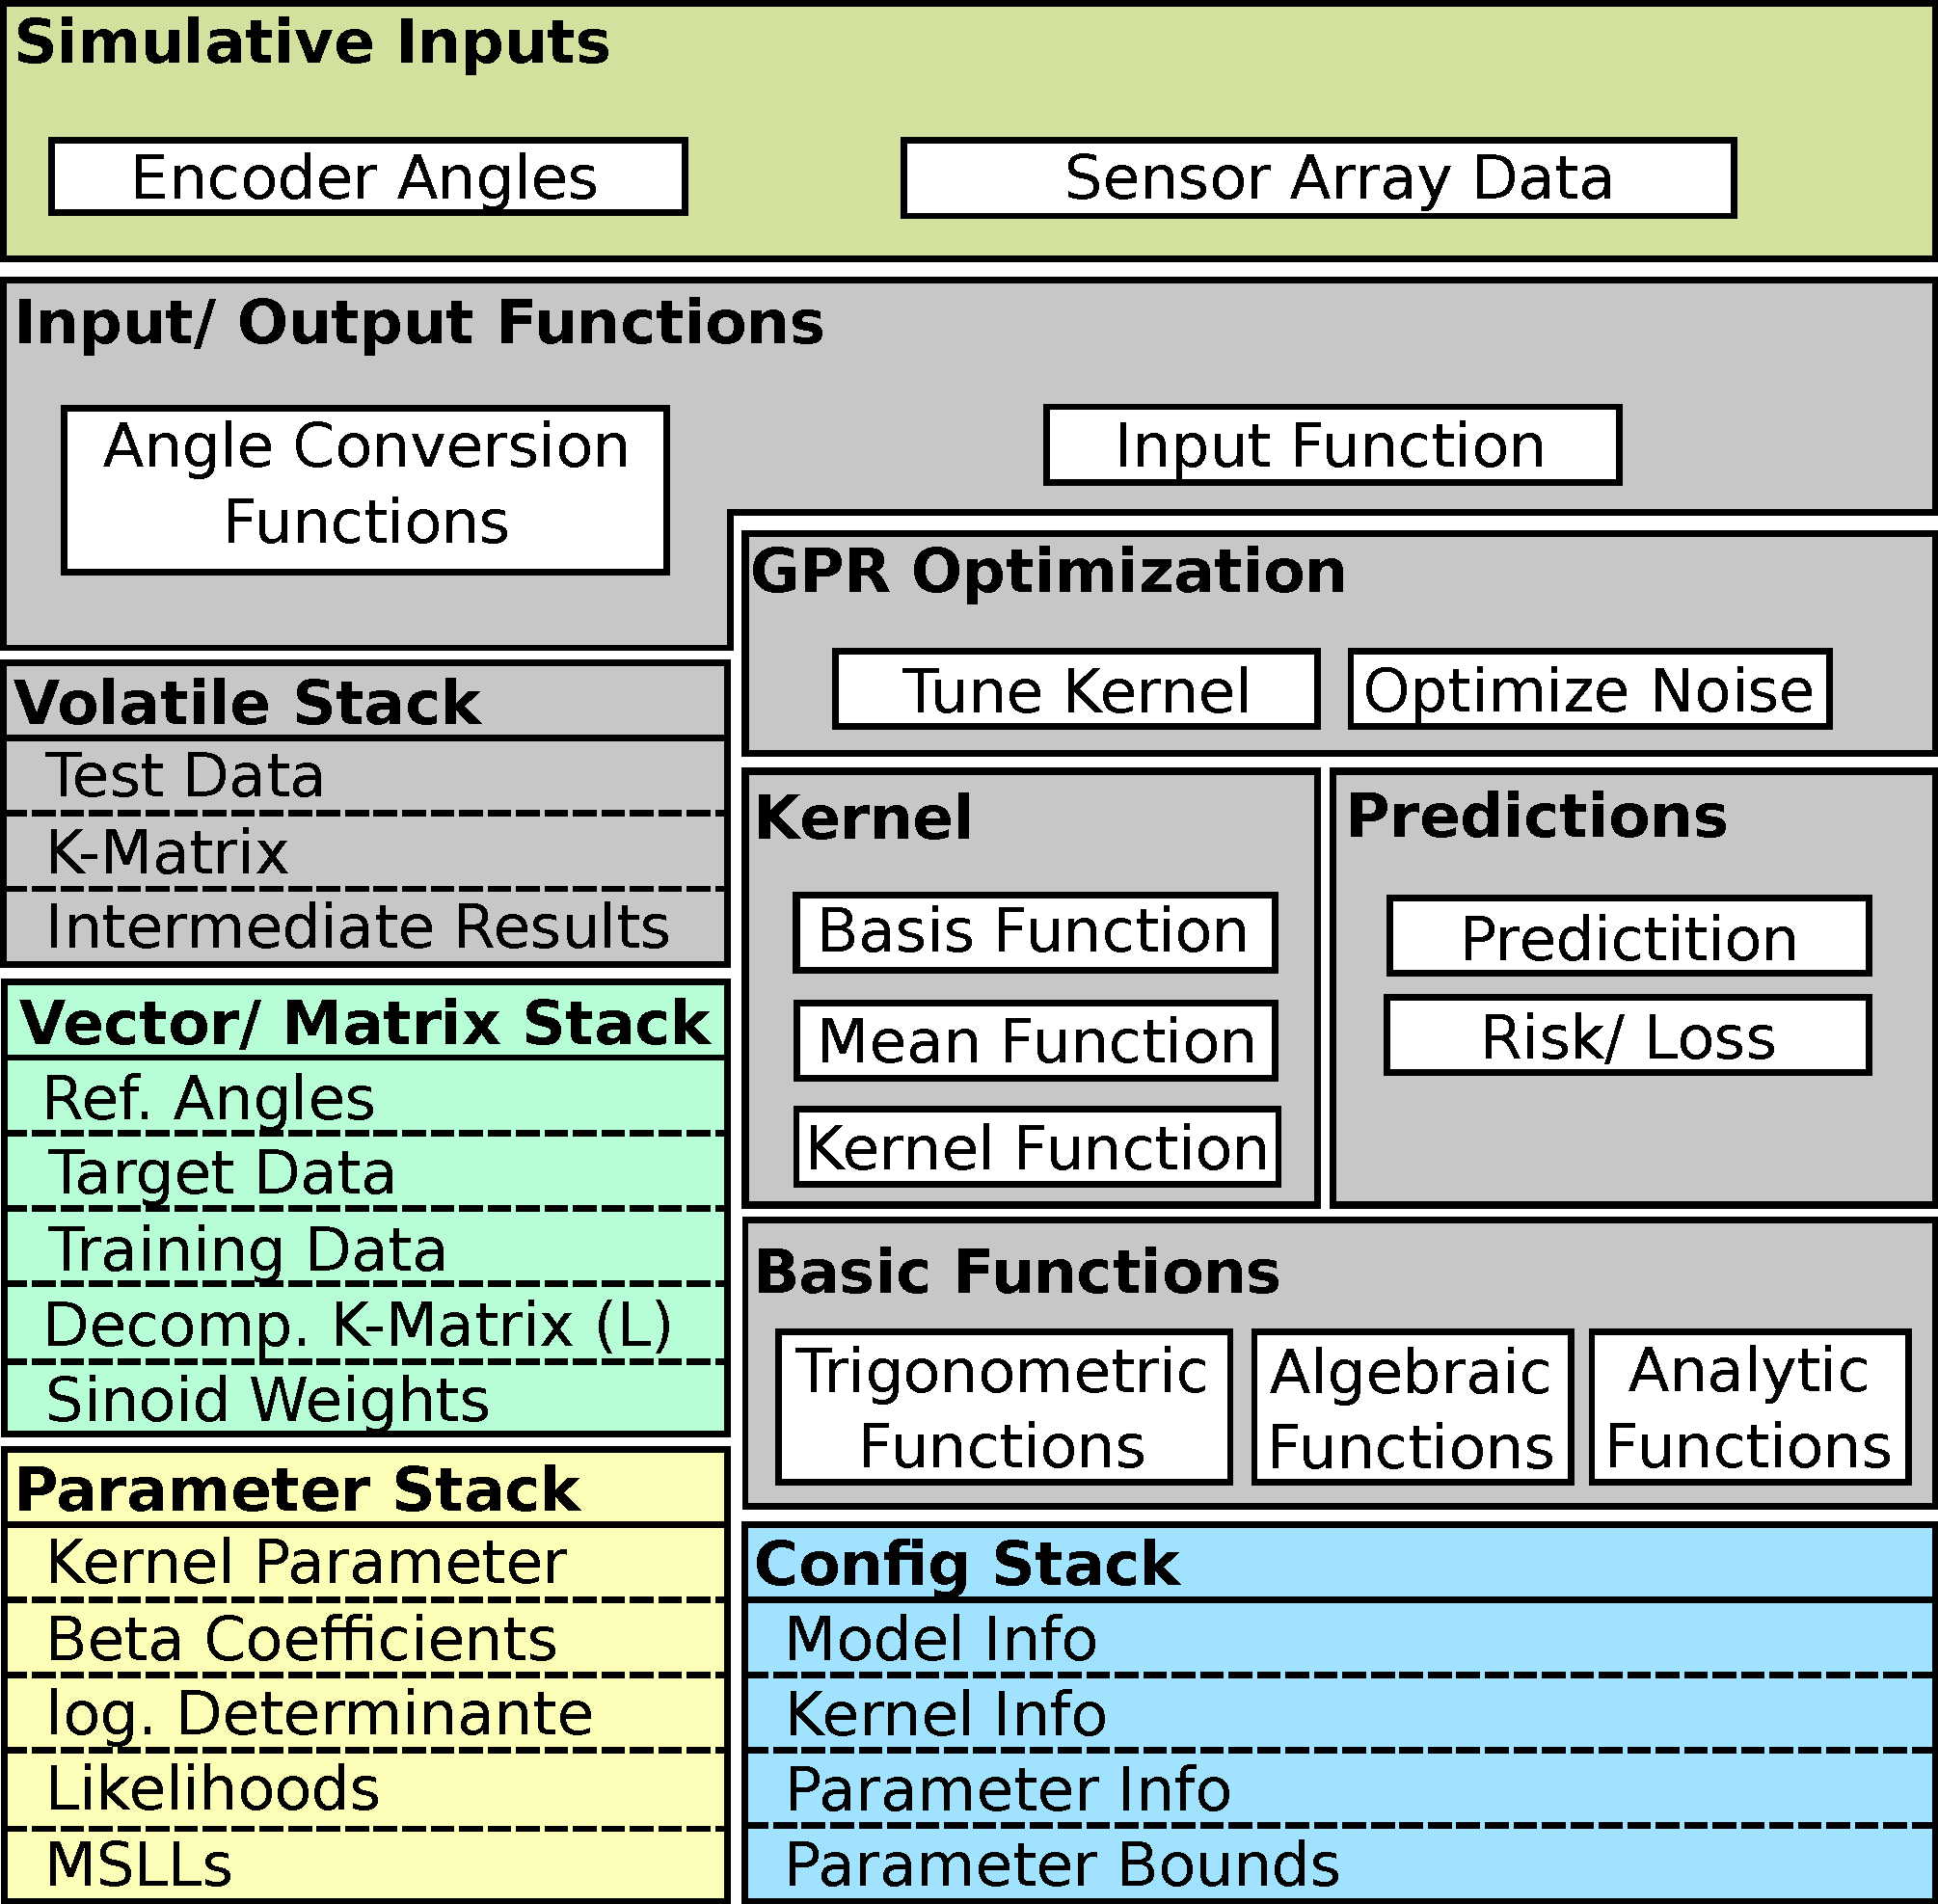
\includegraphics[width=.7\linewidth]{chapters/images/3-SW-E-OExp/Blockschema_Trainingsphase}
	\caption[Blockschema Trainingsphase Regression]{Blockschema Trainingsphase Regression. Veranschaulichung des Funktionsaufrufs für die Trainingsphase in einem Skript. Basierend auf übergebenen Konfigurations-Stack werden Modellfunktionalität aus Submodulen geladen und im Struct-Modell via Funktions-Handles verlinkt. Eingespeistes Trainings- und Testdatensatzpaar dient zur schrittweisen Modellinitialisierung und -Optimierung. Sich einstellende Parameterkonfigurationen werden mit Trainingsdaten als Stacks abgelegt. Resultierendes Struct-Modell enthält alle für Winkelvorhersagen nötigen Daten sowie Parameter und ihren Grenzen (engl. parameter bounds) aus der Optimierung.}
	\label{fig:blockschematrainingsphase}
\end{figure}


\clearpage


Die Trainingsphase ist sehr aufwendig in ihrer Umsetzung und daher in Teilprozessschritte realisiert. \autoref{fig:gproptimization} zeigt den Hauptprozessablauf mit Weiterleitung zu den Teilprozessen in \autoref{fig:noiseoptimization} und \autoref{fig:kerneltuning}. Nach Übergabe der Regressionskonfiguration sowie der Trainings- und Testdaten, wird das Regressionsmodell in einem Struct initialisiert, siehe Funktion im \autoref{mcode:initgpr} und \autoref{fig:gprinitialization}.

\vspace{5mm}
\begin{figure}[bph]
	\centering
	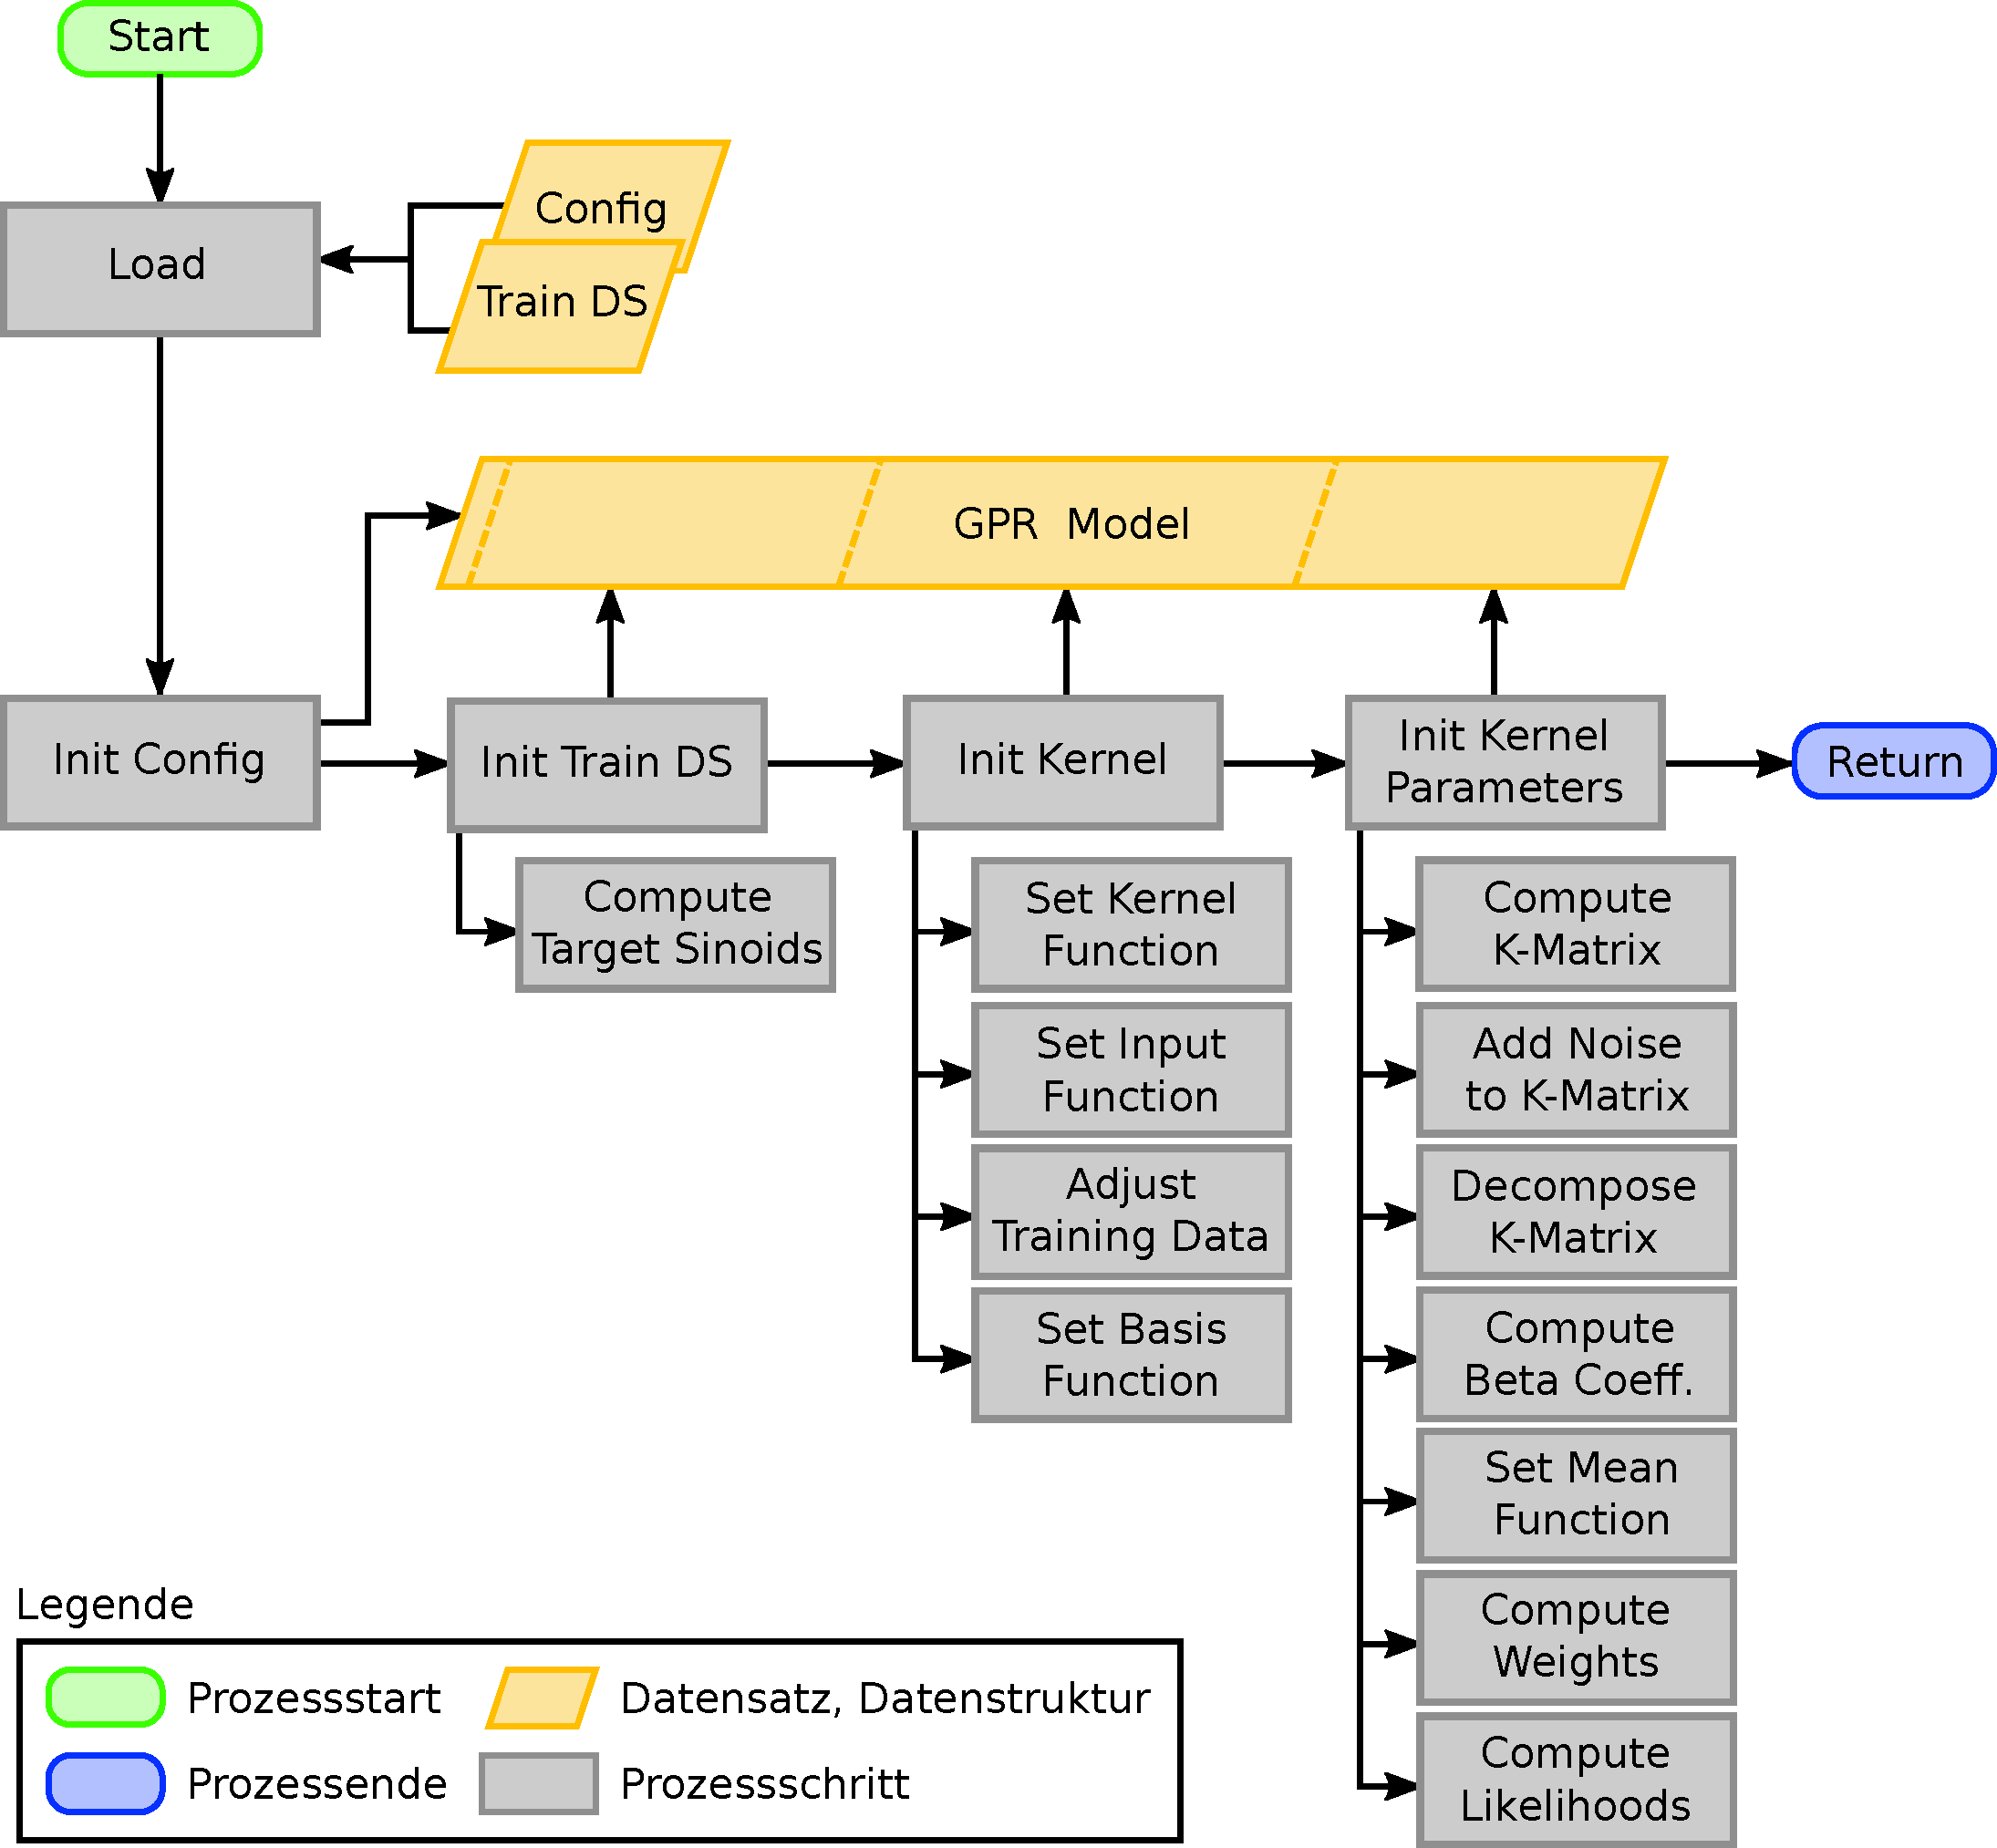
\includegraphics[width=\linewidth]{chapters/images/3-SW-E-OExp/GPR_Initialization}
	\caption[Regressionsinitialisierung Prozessansicht]{Regressionsinitialisierung Prozessansicht. Nach \autoref{alg:gprinit} in mehreren Teilschritten. Konfiguration, Trainingsdatensatz, Kernel-Module und abschließende Regressionsinitialisierung sind mit Funktionen aus \autoref{mcode:initgproptions} bis \autoref{mcode:initkernelparameters} realisiert.}
	\label{fig:gprinitialization}
\end{figure}


\clearpage


Anschließend wird nach eingestellter Konfiguration die Rauschniveauoptimierung mittels der Matlab BayesOpt-Funktion initialisiert. Dazu werden entsprechende Berechnungen auf den Testdaten mit der Funktion aus \autoref{mcode:computeoptimcriteria} umgesetzt. Für jedes ausprobierte Rauschniveau folgt eine Optimierung des Modells nach \autoref{fig:kerneltuning} und eine darauffolgende Berechnung Modellverluste mittels Funktion aus \autoref{mcode:lossds}. Das Gesamtverfahren über die BayesOpt-Funktion ist ein Standardverfahren, dass durch Probieren sich einer optimalen Lösung annähert. Es werden ausprobierte Rauschniveaus und evaluierte Verluste nach \autoref{eq:bayesopt} und \autoref{alg:bayesopt} über alle Versuchsdurchläufe zwischengespeichert. Nach erreichen der eingestellten Durchlaufzahl für die Rauschniveauoptimierung mittels BayesOpt-Funktion, gibt die BayesOpt-Funktion alle ausprobierten Niveaus und errechneten Modellverluste in einem Result-Objekt zurück. Aus dem Result-Objekt werden für die finale Feinabstimmung das gefundene Rauschniveau am Minimum der aufgezeichneten Modellverluste entnommen.


\vspace{5mm}
\begin{figure}[tbph]
	\centering
	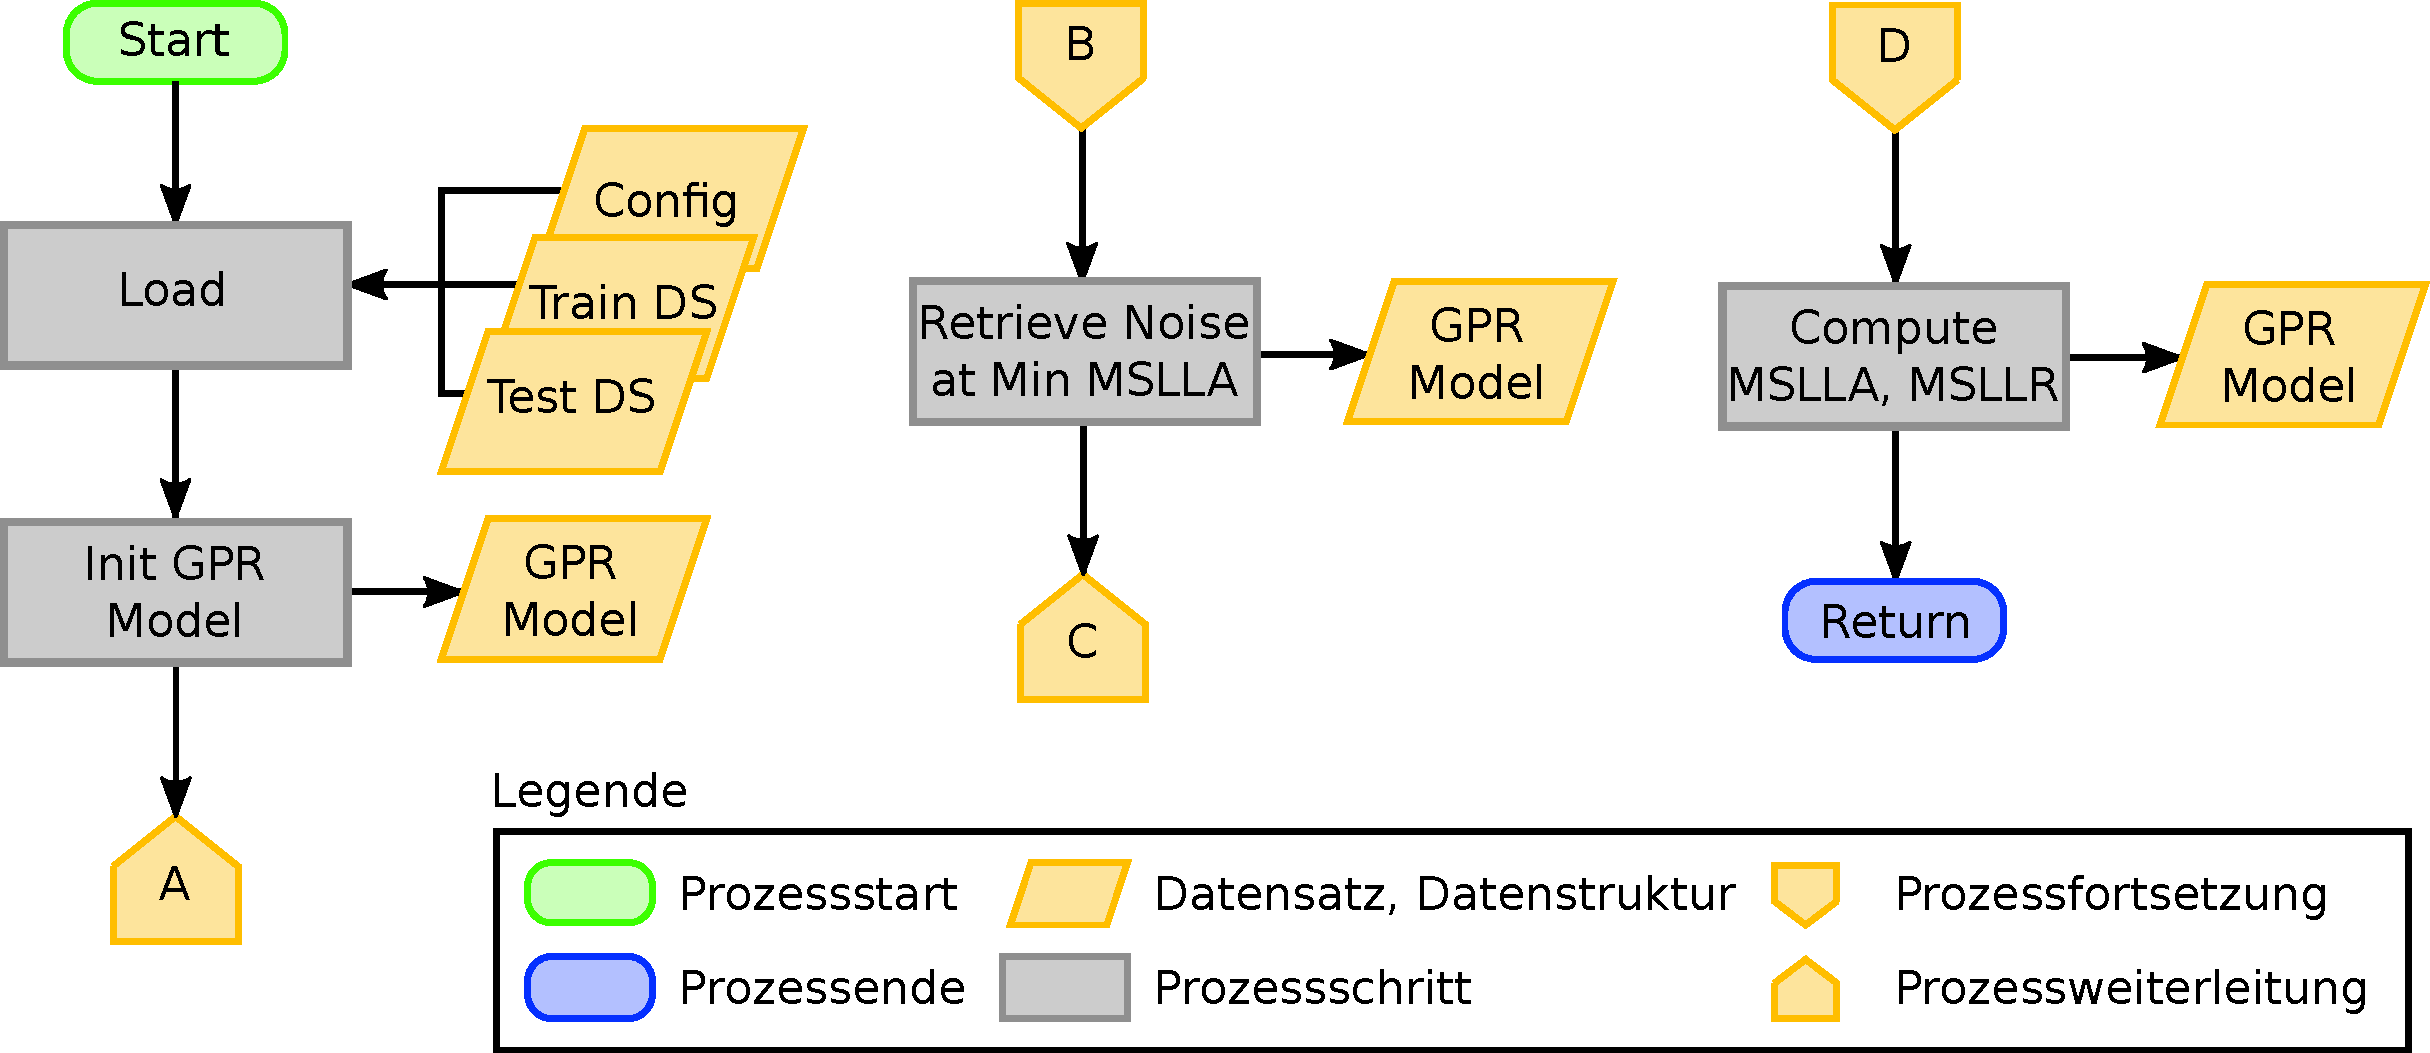
\includegraphics[width=\linewidth]{chapters/images/3-SW-E-OExp/GPR_Optimization}
	\caption[Regressionsoptimierung/ -Generalisierung Prozessansicht]{Regressionsoptimierung/ -Generalisierung Prozessansicht. Darstellung \autoref{alg:bayesopt} Teilprozessschritte. Modellinitialisierung in \autoref{fig:gprinitialization}. Rauschoptimierung (A, B in \autoref{fig:noiseoptimization}) und finale Feinabstimmung (C, D in \autoref{fig:kerneltuning}).}
	\label{fig:gproptimization}
\end{figure}


\clearpage


Dieser Prozess wird innerhalb der BayesOpt-Funktion wiederholt, bis die eingestellte maximale Durchlaufzahl erreicht ist. Wird zu früh abgebrochen, kann bei falsch gewählten Parametergrenzen (engl. parameter bounds) keine hinreichend genaue Lösung gefunden werden. Daher ist die Durchlaufzahl bei weiten Parameter-Bounds entsprechend hoch zu wählen, sodass der Algorithmus genügend Versuche hat schlechte Wertebereiche auszuschließen.


\vspace{5mm}
\begin{figure}[bph]
	\centering
	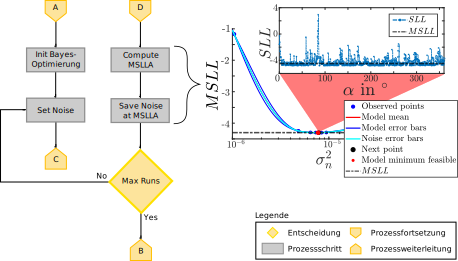
\includegraphics[width=\linewidth]{chapters/images/3-SW-E-OExp/Noise_Optimization}
	\caption[Rauschniveauoptimierung Prozessansicht]{Rauschniveauoptimierung Prozessansicht. Kernprozess in \autoref{alg:bayesopt} bzw. \autoref{fig:gproptimization}. Löst Min-Kriterium nach \autoref{eq:bayesopt}. Die Berechnung ist als Funktions-Handle von \autoref{mcode:computeoptimcriteria} der BayesOpt-Funktion zu übergeben. Die Rauschniveauoptimierung misst durch Probieren das Rauschniveau $\sigma_n^2$ gegenüber dem mittleren Modellverlust $MSLL$. Zwischenprozess ist die Parameteroptimierung (C, D) in \autoref{fig:kerneltuning}}
	\label{fig:noiseoptimization}
\end{figure}


\clearpage


Der Zwischenprozessschritt zur inneren Parameteroptimierung nach \autoref{fig:kerneltuning} ist in der Funktion \autoref{mcode:tunekernel} implementiert. Diese bedient sich der Matlab Fmincon-Funktion um \autoref{alg:fminconopt} zu lösen. Das aufzulösende Min-Kriterium aus \autoref{eq:fmincon} wird der Fmincon-Funktion als Funktions-Handle bereitgestellt. Das Min-Kriterium wird mittels der Funktion aus \autoref{mcode:computetunecriteria} berechnet. Dabei wird das Regressionsmodell z.T. reinitialisiert. Dieser Prozessschritt wird auch zur finalen Feinabstimmung mit optimiertem Rauschniveau genutzt. Nach Abarbeitung aller Optimierungsprozesse steht das fertige Regressionsmodell als Eingabeargument für die Arbeitsphase bereit.


\vspace{5mm}
\begin{figure}[bph]
	\centering
	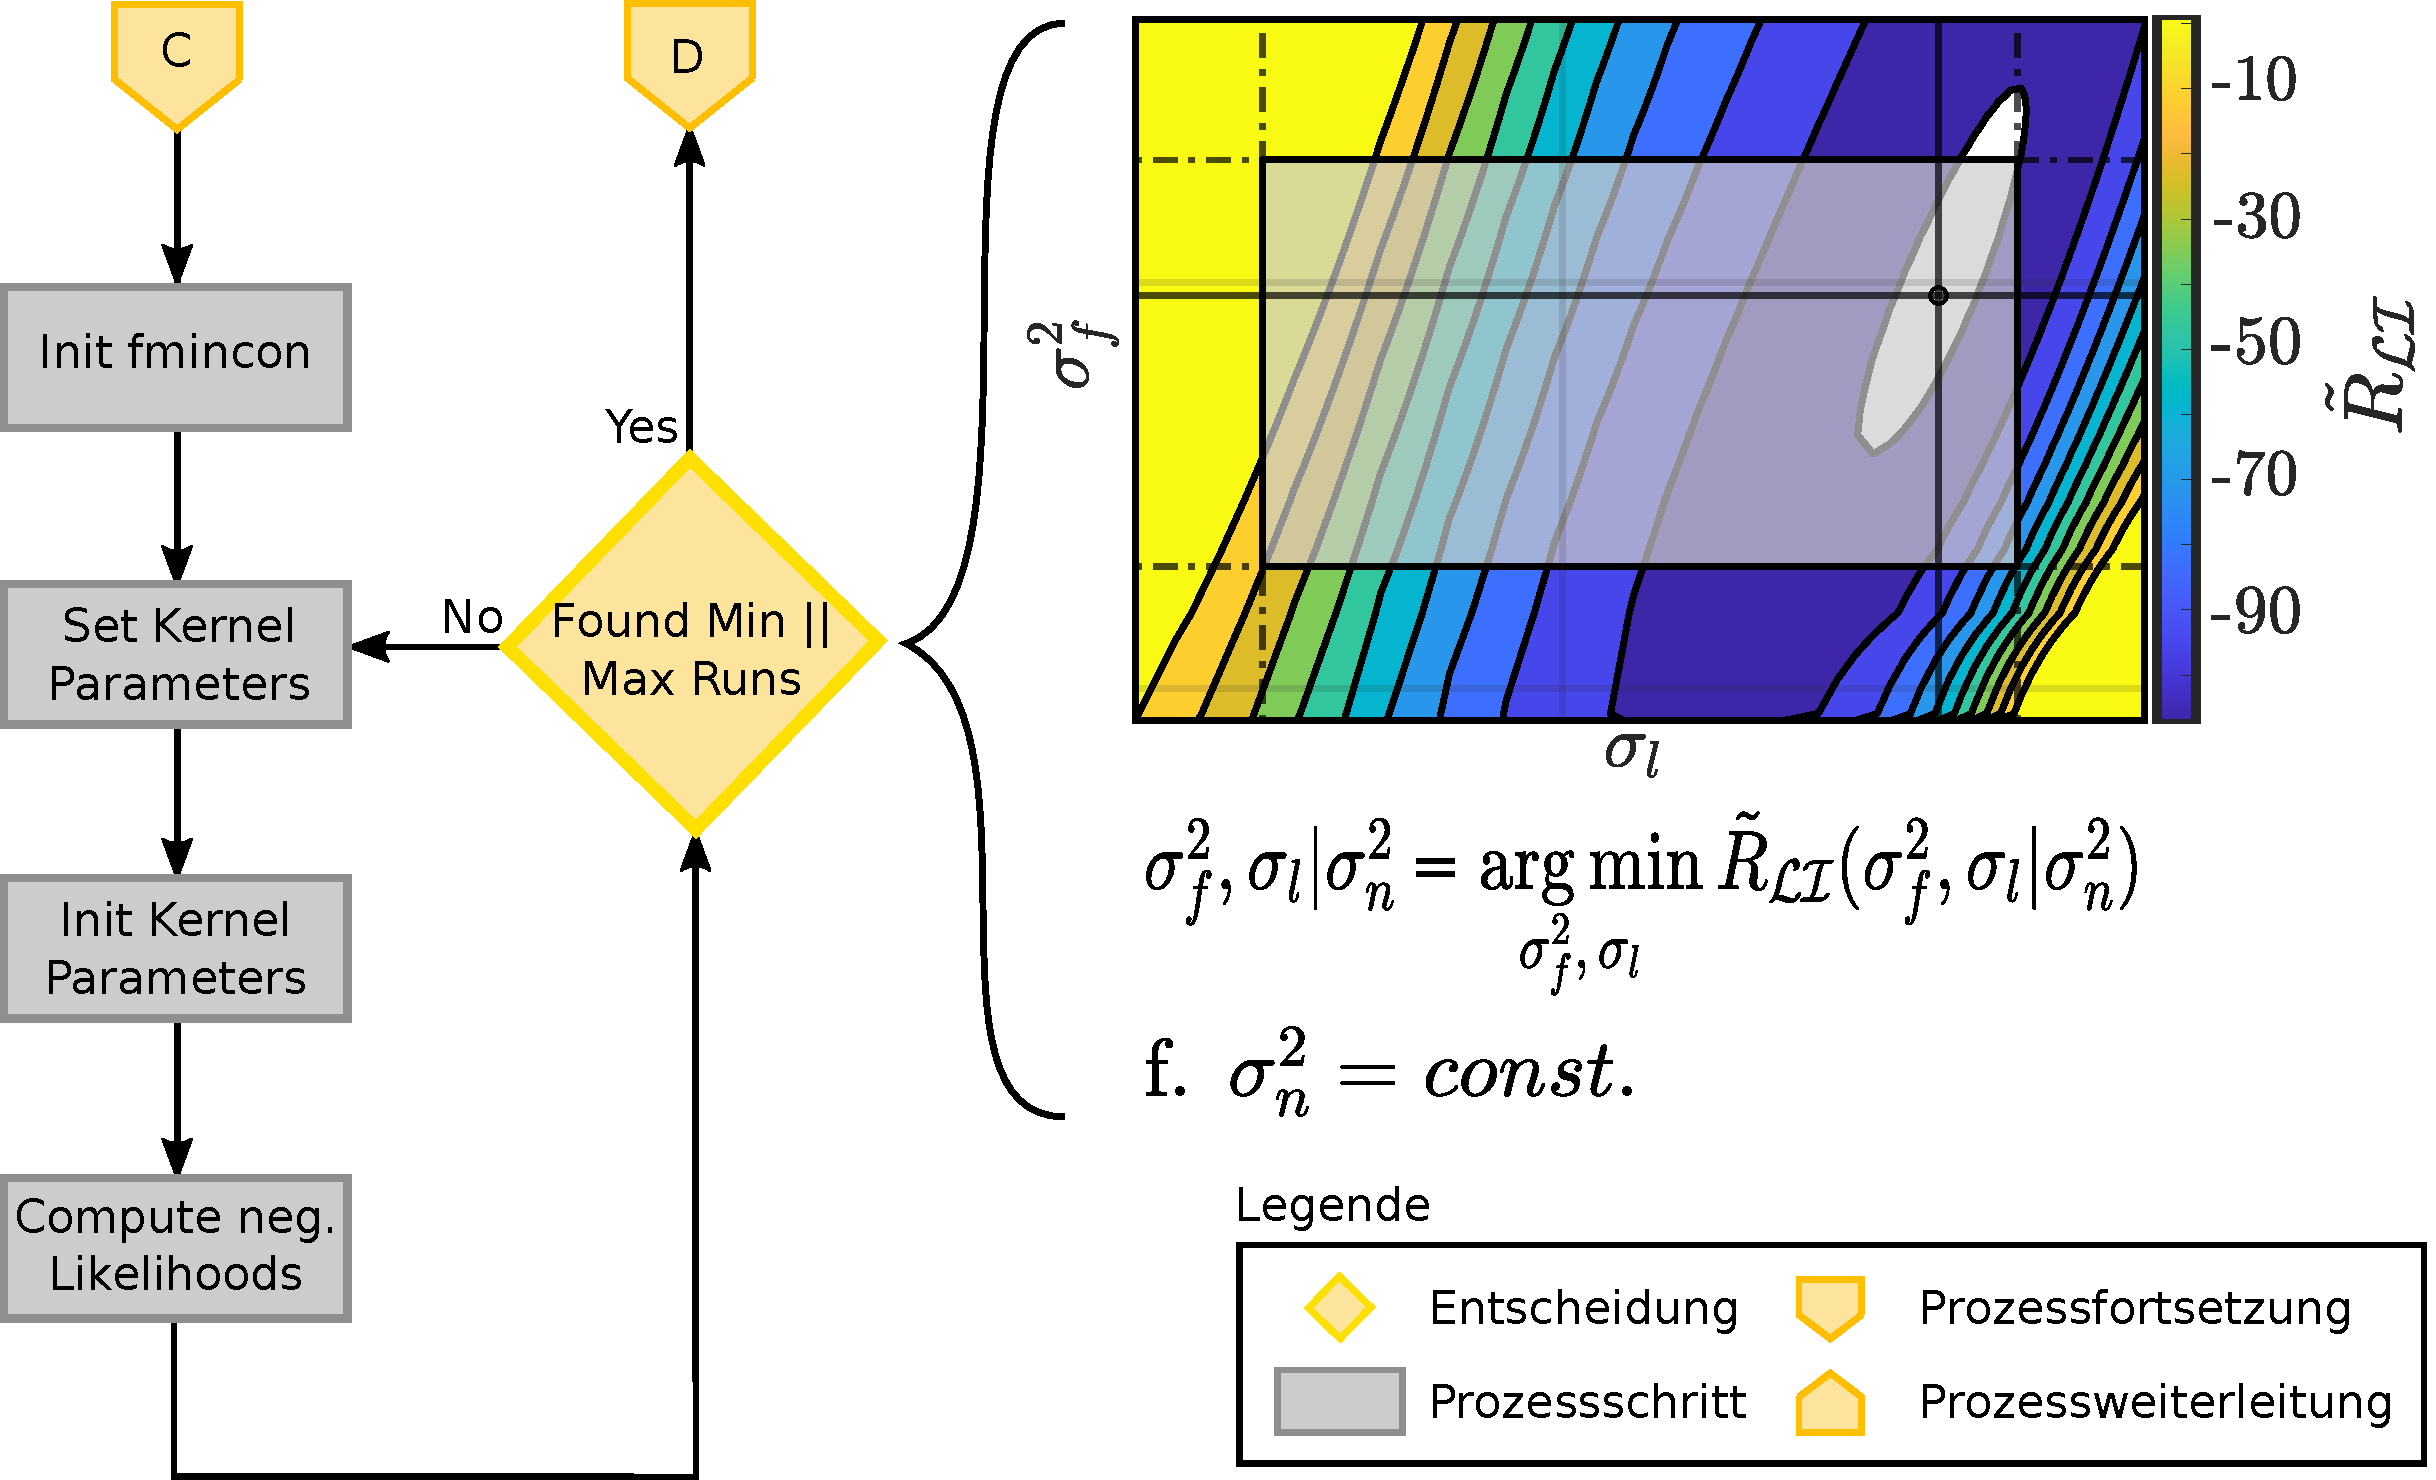
\includegraphics[width=\linewidth]{chapters/images/3-SW-E-OExp/Kernel_Tuning}
	\caption[Regressionsparameteroptimierung Prozessansicht]{Regressionsparameteroptimierung Prozessansicht. Lösung des \autoref{alg:fminconopt} mittels Matlab Fmincon-Funktion. Das Min-Kriterium aus \autoref{eq:fmincon} ist als Funktion in \autoref{mcode:computetunecriteria} als Funktions-Handle an die Fmincon-Funktion zu übergeben. Die Parameteroptimierung für die Kovarianzfunktion $\theta = (\sigma_f^2,\sigma_l)$ sucht, in einem durch Parameter-Bounds eingeschränkten Areal, nach lokalem Minimum $\tilde{R}_{\mathcal{L}}$ bei logarithmisch gegeneinander aufgetragenen Parameterkombination für $\sigma_f^2$ und $\sigma_l$.}
	\label{fig:kerneltuning}
\end{figure}


\clearpage


\paragraph{Arbeitsphase}\label{par:gpr-work-pro}$~$\\


Die Einbindung der Arbeitsphase ist im Vergleich zur Trainingsphase trivial. Das fertig optimierte Struct-Model wird einfach zusammen mit einem kompletten Testdatensatz der Vorhersage-Funktion aus \autoref{mcode:predds} und der Verlustfunktion aus \autoref{mcode:lossds} übergeben. Berechnete Vorhersagen und Verluste stehen dann gemäß \autoref{sec:gprpred} als Ergebnisvektoren bereit und können zur weiteren Auswertung genutzt werden.


\vspace{5mm}
\begin{figure}[tbph]
	\centering
	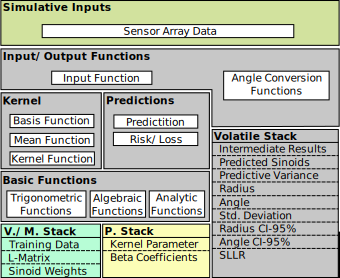
\includegraphics[width=0.7\linewidth]{chapters/images/3-SW-E-OExp/Blockschema_Workphase}
	\caption[Blockschema Arbeitsphase Regression]{Blockschema Arbeitsphase Regression. Das fertig optimierte Modell wird mit minimalem Parameterbetrieb in Vorhersage- und Verlustfunktion als Argument zusammen mit den Testdaten übergeben. Einbindung ist funktional, siehe \autoref{mcode:predds} und \autoref{mcode:lossds}.}
	\label{fig:blockschemaworkphase}
\end{figure}

